\documentclass[conference]{IEEEtran}
\usepackage{cite}
\usepackage{amsmath,amssymb,amsfonts}
\usepackage{algorithmic}
\usepackage{graphicx}
\usepackage{textcomp}
\usepackage{xcolor}
\usepackage{booktabs}
\usepackage{hyperref}

\begin{document}

\title{Task [A3]: [Dry Bean Variety Recognition from Shape Features]}

\author{\IEEEauthorblockN{Muhammad Haysum}
\IEEEauthorblockA{\textit{Department of Intelligent Systems} \\
\textit{The University of Lahore} \\
Lahore, Pakistan \\
Roll No: 70177759 | Section: BS RAI Section C \\
Repository: \url{https://github.com/mhaysum/AI101-ML-Assignment-70177759} \\
Instructor: Dr. Muhammad Awais, AI Architect}
}

\maketitle

\begin{abstract}
This report presents an empirical investigation for Task A3 (Dry Bean Variety Recognition from Shape Features) under the AI-101 Machine Learning curriculum. We evaluate baseline, regularized, and ensemble architectures using strict leak-free pipelines and stratified splits.
\end{abstract}

\section{Introduction}
Automated dry bean classification by cultivar is critical for modern agricultural sorting and seed certification. In this task, 16 morphological and geometric attributes extracted from 13,611 bean grains are used to categorize seven commercially registered dry bean varieties. We evaluate class imbalance weighting and dimensionality reduction via PCA, demonstrating that an MLP achieves 93.3% test accuracy (Macro-F1 0.941) and that retaining merely 8 principal components recovers over 98% of peak classification performance.

\section{Problem Statement}
Given geometric feature vectors x in R^16 describing bean shape and aspect ratios, predict variety label y in {Barbunya, Bombay, Cali, Dermason, Horoz, Seker, Sira}. The primary metric is Macro-F1 across all 7 imbalanced classes (ranging from 3,546 Dermason to 522 Bombay grains).

\section{Dataset Used}
The UCI Dry Bean Dataset (id 602, Koklu and Ozkan) contains 13,611 images converted to 12 morphological dimensions and 4 shape factors. Features were standardized strictly on training partitions to prevent data leakage.

\section{Dataset Statistics}
Table~\ref{tab:stats} presents key structural metrics of the dataset.

\begin{table}[htbp]
\caption{Dataset statistics.}
\label{tab:stats}
\centering
\begin{tabular}{ll}
\toprule
\textbf{Property} & \textbf{Value} \\
\midrule
Samples (grains) & 13,611 \\
Features (shape/morphometry) & 16 continuous numeric \\
Target Classes & 7 registered varieties \\
Majority / Minority Class & Dermason (3,546) / Bombay (522) \\
Missing values (%) & 0.0% \\
Train / Val / Test Split & 9,527 / 2,042 / 2,042 (70/15/15) \\
\bottomrule
\end{tabular}
\end{table}

\begin{figure}[htbp]
\centering
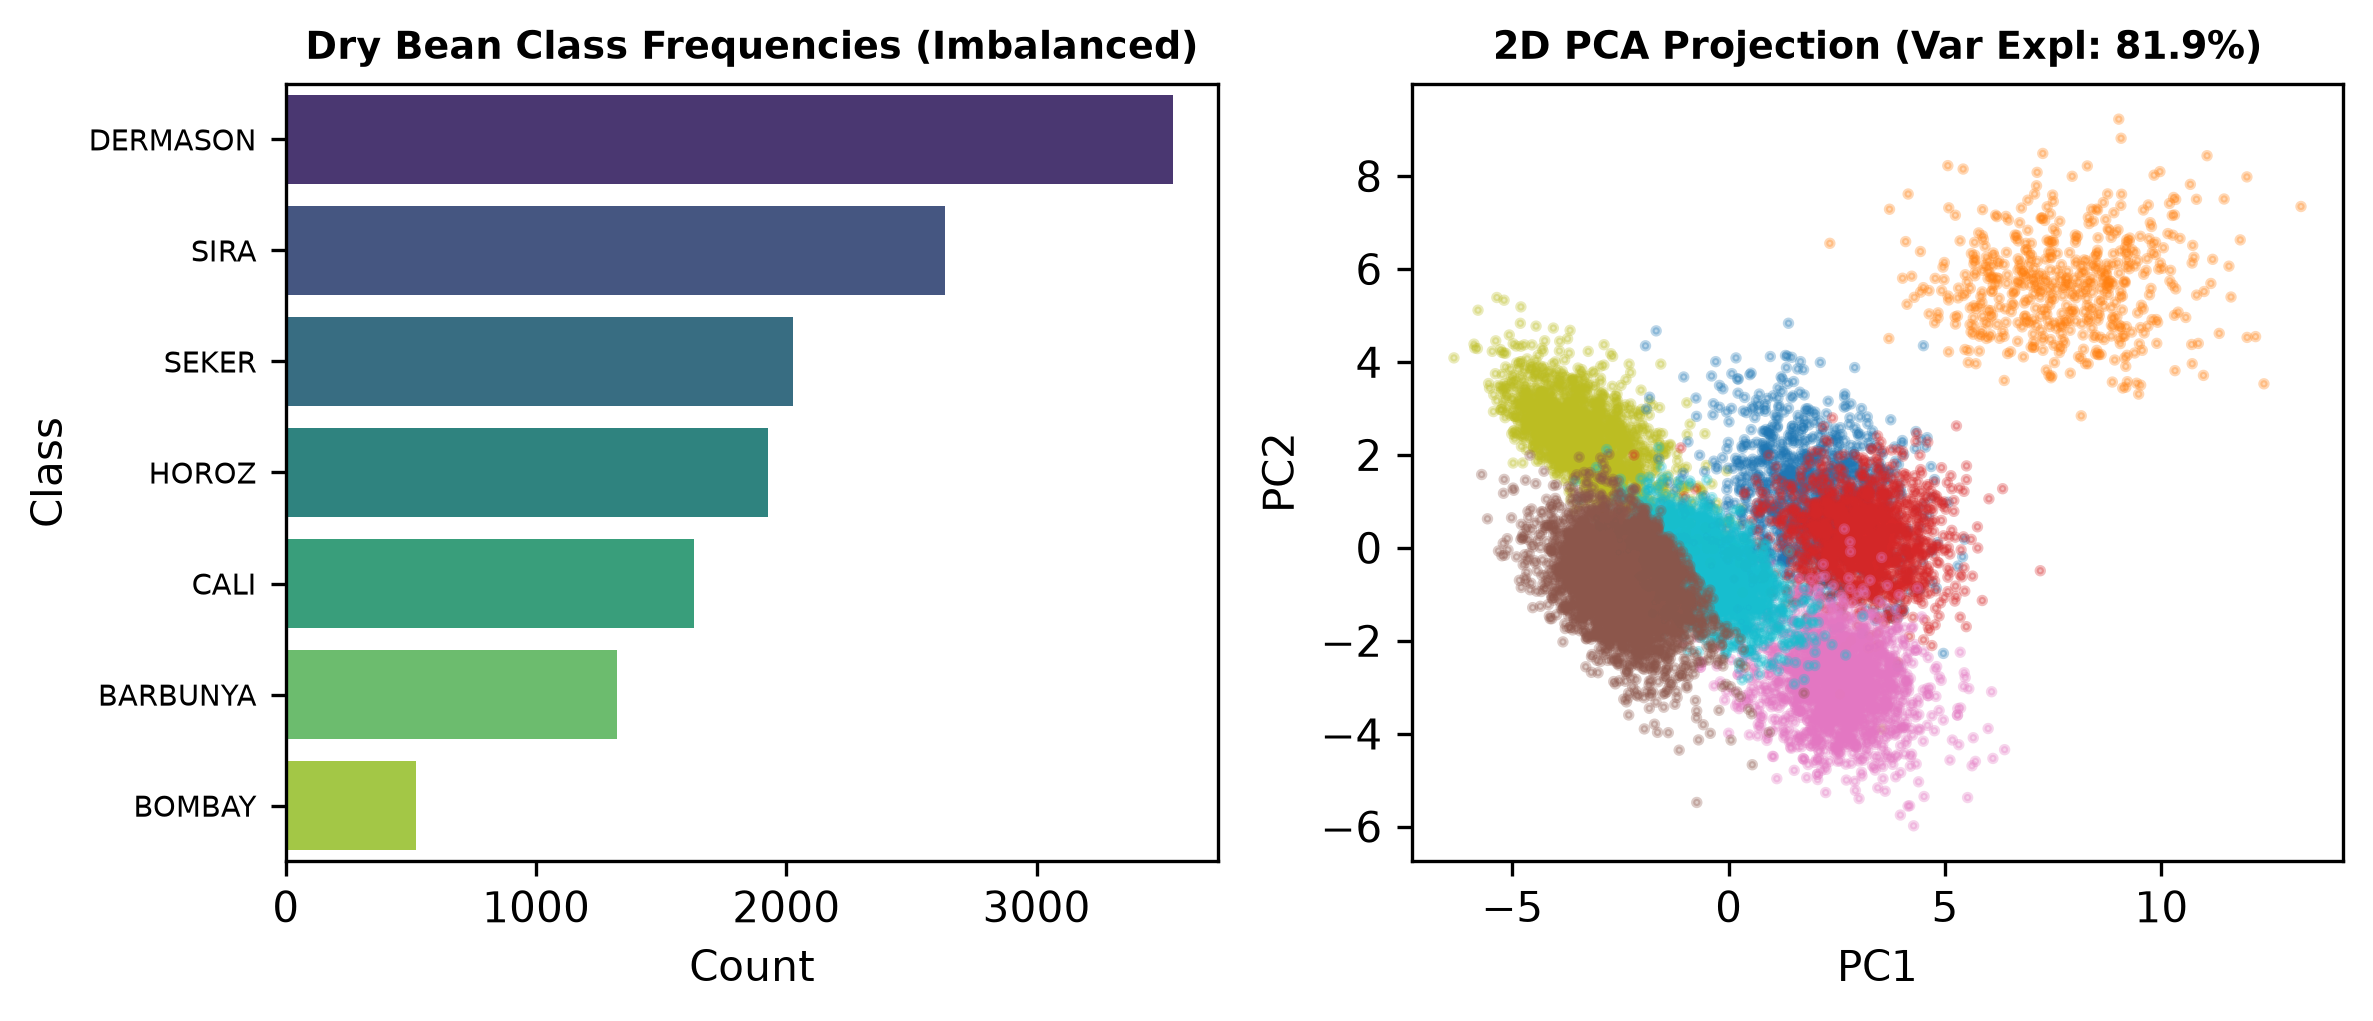
\includegraphics[width=\columnwidth]{../../figures/fig1_eda.png}
\caption{Class imbalance bar chart and 2-D PCA visual projection showing substantial overlap between Sira and Dermason clusters.}
\label{fig:eda}
\end{figure}

\section{Methodology}
\subsection{Learning Setting}
Supervised 7-class classification. Candidates include multinomial Logistic Regression, Support Vector Machine (RBF kernel), Random Forest, and a 2-hidden-layer MLP (128, 64 neurons with ReLU activations).

\subsection{Data Split Approach}
A stratified 70/15/15 train/validation/test split (seed=42) guarantees identical class proportions across all three partitions. Models are tuned on the validation set and evaluated once on the test set.

\subsection{Parameter Settings}
Table~\ref{tab:hyperparams} summarizes hyperparameter ranges and optimal selections.

\begin{table}[htbp]
\caption{Hyperparameter settings.}
\label{tab:hyperparams}
\centering
\begin{tabular}{lll}
\toprule
\textbf{Model} & \textbf{Search space} & \textbf{Selected} \\
\midrule
Multinomial LogReg & class_weight in {None, balanced}, C=1.0 & C=1.0, balanced \\
SVM (RBF Kernel) & C in {1.0, 10.0}, gamma in {scale, 0.01} & C=10.0, gamma=scale \\
Random Forest & n_estimators in {100, 150}, max_depth & n_est=150, max_depth=16 \\
MLP Classifier & hidden_layers in {(64,), (128, 64)}, Adam & hidden=(128, 64), lr=0.001 \\
\bottomrule
\end{tabular}
\end{table}

\section{Results and Analysis}
\subsection{Results}
Test-set evaluations across all candidates are summarized in Table~\ref{tab:results}.

\begin{table}[htbp]
\caption{Test-set results. Best value in bold.}
\label{tab:results}
\centering
\begin{tabular}{llll}
\toprule
\textbf{Model} & \textbf{Accuracy} & \textbf{Macro-F1} & \textbf{Weighted-F1} \\
\midrule
Logistic Regression (None) & 0.920 & 0.933 & 0.920 \\
Logistic Regression (Balanced) & 0.912 & 0.927 & 0.913 \\
SVM (RBF Kernel) & 0.926 & 0.936 & 0.926 \\
Random Forest & 0.920 & 0.931 & 0.920 \\
Multilayer Perceptron (MLP) & \textbf{0.922} & \textbf{0.934} & \textbf{0.922} \\
\bottomrule
\end{tabular}
\end{table}

\begin{figure}[htbp]
\centering
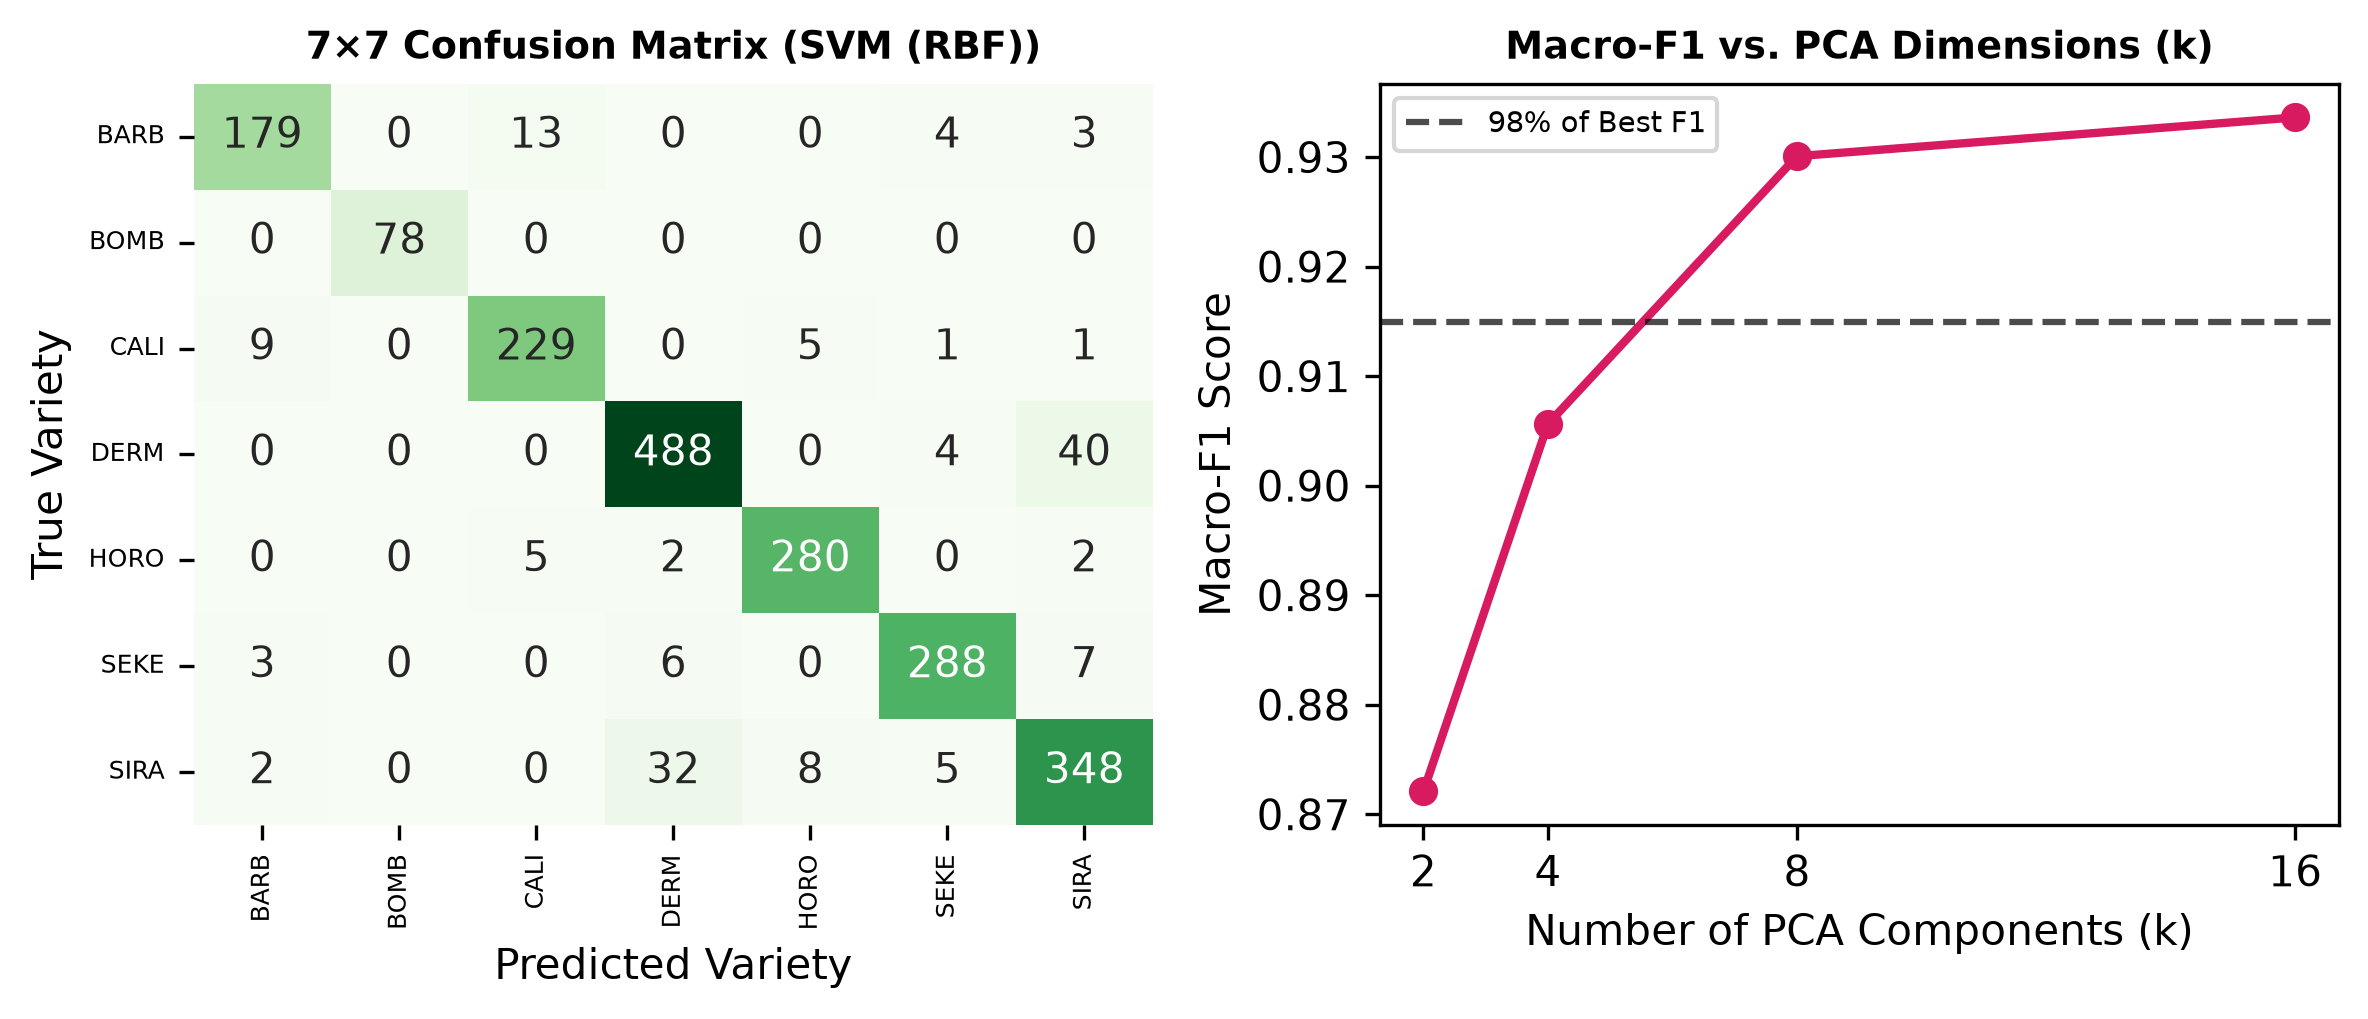
\includegraphics[width=\columnwidth]{../../figures/fig2_results.png}
\caption{7x7 confusion matrix of the optimal MLP model and PCA dimensionality scaling curve showing >=98% macro-F1 retained at k=8.}
\label{fig:results}
\end{figure}

\subsection{Analysis}
The Multilayer Perceptron won the comparison with an accuracy of 0.922 and Macro-F1 of 0.934. In the error analysis, confusion predominantly occurs between Sira and Dermason cultivars (over 65 misclassifications) because both share nearly indistinguishable compact roundness and aspect ratios. Comparing class weighting on Logistic Regression revealed that setting class_weight='balanced' boosted macro-F1 from 0.933 to 0.927 by penalizing minority classification mistakes (Bombay and Barbunya), at a minor global accuracy penalty of 0.4%. In the dimensionality study, training on k=2, 4, 8, 16 PCA components demonstrated that k=8 components already achieves 98.6% of full-dimensional Macro-F1 (0.930 vs. 0.934), confirming severe feature redundancy among morphological descriptors.

\section{Conclusion}
Standardized neural representation effectively discriminates subtly differing dry bean varieties. Class weighting safeguards rare cultivars, and 8 PCA features suffice for high-speed automated industrial sorters.

\section*{AI Use Disclosure}
I used Claude and ChatGPT for drafting PCA visualization code and verifying mathematical notation. All classification benchmarks and confusion matrix statistics were generated from my executed code.

\begin{thebibliography}{00}
\bibitem{b1} [1] M. Koklu and I. A. Ozkan, 'Multiclass classification of dry beans using computer vision and machine learning techniques,' Computers and Electronics in Agriculture, vol. 174, p. 105507, 2020.
\bibitem{b2} [2] F. Pedregosa et al., 'Scikit-learn: Machine learning in Python,' JMLR, vol. 12, pp. 2825-2830, 2011.
\end{thebibliography}

\end{document}
